\chapter{Introduzione}
\label{chap:fond}

\begin{minipage}{12cm}\textit{Se lo si desidera, utilizzare questo spazio per inserire un breve riassunto di ci\`o che verr\`a detto in questo capitolo. Inserire solo i punti salienti.}
\end{minipage}

\vspace*{1cm}

\section{Obiettivo/ Research question}

Scrivere obiettivo e research question

\section{Stato dell'arte}
\subsection{Speeded Up Robust Feature}
\label{sec:iniziare}

L'algoritmo SURF (Speeded Up Robust Feature) \`e un descrittore e un detector
robusto di caratteristiche locali di un'immagine.
\`E diverse volte pi\`u veloce e robusto di SIFT, il descrittore a cui si
ispira.
 SURF \`e stato presentato nel 2006 da Hebert Bay e ne sono state realizzate
 diverse implementazioni open source e commerciali:
l'implementazione originale (commerciale) \`e scritta in c++, mentre
{\itshape JavaSurf}, {\itshape JopenSURF}, {\itshape ImageJ SURF} e {\itshape
BoofCV} sono implementazioni open source per Java.

Per cercare corrispondenze tra immagini in genere si procede con tre passi fondamentali:
\begin {enumerate}
  \item Si individuando i ``punti di interesse'' (ad esempio i bordi) che hanno
  la caratteristica di ripetersi, ossia possono essere ritrovati da un detector anche se cambia la prospettiva 
  di visualizzazione dell'immagine.
  \item Si descrivono i punti di interesse tramite un vettore di
  caratteristiche. Questo vettore deve essere di grandi dimensioni se si intende
  privilegiare la robustezza dell'algoritmo oppure di piccole dimensioni se
  l'obiettivo \`e la velocit\`a computazionale.
  \item Si effettua il matching tra i vettori e le immagini.
\end{enumerate}

SURF \`e nato con l'obiettivo di trovare un trade-off tra la velocit\`a
(Speeded-Up) e la robustezza (Robust).
Per l'individuazione e la descrizione dei punti di interesse SURF utilizza l'approssimazione della matrice Hessiana, 
che \`e molto accurata, e le immagini integrali, che riducono drasticamente il
tempo computazionale.

Un'immagine integrale \begin{math} I_{\Sigma}(x,y) \end{math} \`e la somma
dell'intensit\`a dei pixel compresi tra l'origine e il punto di coordinate
\begin{math} (x,y) \end{math}.
In formule:
\begin{displaymath}
I_{\Sigma}(x,y) =\sum_{i=0}^{x} \sum_{j=0}^{y} I(i,j) 
\end{displaymath}

Ottenuta l'immagine integrale bastano quattro operazioni per calcolare un'a\-rea
rettangolare di qualsiasi dimensione. Questa propriet\`a \`e sfruttata da SURF per la realizzazione di filtri di diverse dimensioni.

La matrice Hessiana permette di individuare le strutture �blob� (regioni in cui
propriet\`a come la luminosit\`a e il colore differiscono rispetto a quelle
dell'ambiente) perch\`e in quei punti il determinante (o discriminante) \`e
massimo, e di selezionare la scala dell'immagine; tuttavia le immagini con rotazioni di multipli dispari di \begin{math} \frac{\pi}{4} \end{math} perdono
ripetibilit\`a.
Le risposte blob sono memorizzate in una mappa di risposte su scale differenti.

\`E fondamentale poter trovare i punti di interesse della stessa immagine su diverse scale 
poich\`e spesso si cercano corrispondenze tra due immagini rappresentate con
scale diverse.
Lo spazio delle scale pu\`o essere rappresentato come una piramide; con i
metodi tradizionali (ad esempio SIFT) l'immagine viene continuamente ridimensionata mentre SURF ridimensiona solo il filtro: il calcolo delle scale 
pu\`o essere eseguito con attivit\`a in parallelo guadagnando velocit\`a
computazionale mentre con SIFT l'immagine ad ogni livello di scala dipende da quella precedente, per cui la computazione \`e sequenziale. La differenza 
tra i metodi SIFT e SURF \`e mostrata in Figura 1.1.

\begin{figure}[htbp]
\centering
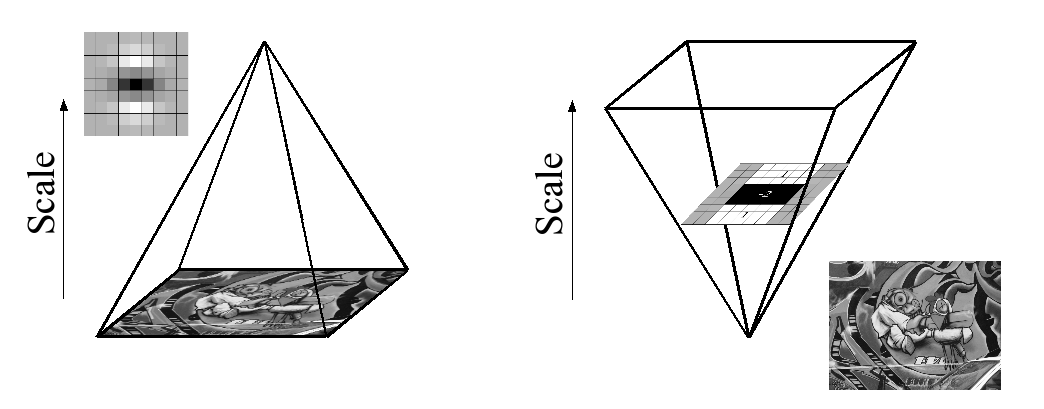
\includegraphics[scale=0.2]{Image/Figura1_1.png}
\caption{A sinistra l'approccio SIFT (ridimensionamento
dell'immagine), a destra il metodo SURF (ridimensionamento del filtro).}
\end{figure}

Il numero di punti di interesse individuati varia con la scala: chiaramente
maggiore \`e la scala minore \`e il numero dei punti di interesse individuati, come mostrato nel seguente diagramma:

\begin{figure}[htbp]
\centering
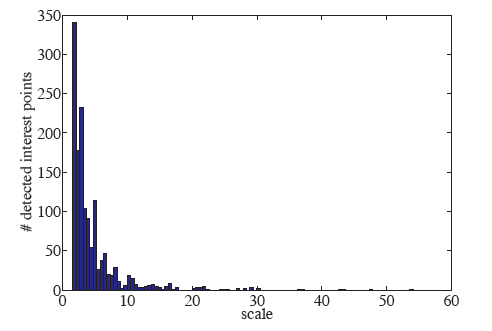
\includegraphics[scale=0.35]{Image/Figura1_2.png}
\caption{Diagramma dei punti di interessi individuati in rapporto alla scala}
\end{figure}

I descrittori SURF descrivono la distribuzione dell'intensit\`a del contenuto (pixel?) nell'intorno del punto 
di interesse in modo simile a SIFT. Si costruisce la distribuzione di primo ordine delle risposte della 
wavelet Haar nelle direzioni x e y e anche in questo caso si utilizzano le immagini integrali per aumentare la velocit\`a.
 
Inizialmente si cerca un'orientazione riproducibile e indipendente dalla rotazione dell'immagine: 
la si ottiene dalle informazioni contenute in una regione circolare intorno al punto di interesse; 
in seguito si costruisce una regione quadrata allineata con l'orientamento trovato e si estrae 
il descrittore SURF composto da 64 componenti; infine si procede con il matching tra le immagini. 
Per quest'ultimo step si cerca di risparmiare tempo distinguendo i blob scuri da quelli chiari e confrontando solo i blob 
che hanno lo stesso tipo di contrasto.

\begin{figure}[htbp]
\centering

\includegraphics[scale=0.4]{Image/Figura1_3.png}
\caption{Due blob con contrasti differenti non sono presi in considerazione per il matching}
\end{figure}

\subsection{Active Shape Models}

I metodi basati su modello utilizzano una forma base che rappresenta
l'immagine; questa viene utilizzata per trovare la  miglior corrispondenza tra
il modello e una nuova immagine.
Questo approccio �top-down� \`e pi\`u semplice e meno soggetto a errori di quello �bottom-up� nel quale l'immagine 
viene analizzata per individuare particolari strutture e punti di interesse che la caratterizzano.

Gli Active shape models (ASMs) sono modelli statistici delle forme di
oggetti che vengono iterativamente deformati fino ad adattarsi alle nuove
immagini.
Sono stati sviluppati da Tim Cootes e Chris Taylor nel 1995.

Il modello ASM \`e costruito in base all'analisi di un training set di immagini
d'esempio e la forma dell'oggetto \`e rappresentato da un insieme di punti controllati dal modello.

L'algoritmo ASM alterna due passi fondamentali:
\begin {enumerate}
  \item La generazione della forma base analizzando l'intorno di ogni punto
  per un miglior posizionamento del punto stesso.
  \item L'adattamento della forma al modello di distibuzione dei punti.
\end{enumerate}

Per il primo passo \`e necessario che l'algoritmo individui dei punti di
riferimento sempre presenti nelle immagini appartenenti al training set: ci\`o
implica che il training set deve contenere la stessa tipologia di oggetti e che questi ultimi abbiano una forma tale da prevedere 
punti di riferimenti ben distinti.

ASM \`e conveniente da utilizzare nel caso in cui:
 \begin{itemize}
   \item Si possiede un insieme di immagini rappresentative del soggetto da rappresentare;
   \item Gli oggetti hanno una forma definita;
   \item Si conosce con buona approssimazione il target dell�immagine.
 \end{itemize}
Nel caso invece di immagini in cui gli oggetti possono assumere forme molto diverse \`e preferibile utilizzare 
un approccio ``bottom-up'' (estrazione delle features).

\begin{figure}[htbp]
\centering
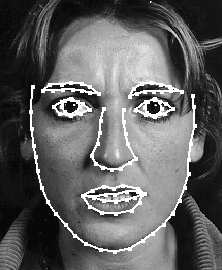
\includegraphics[scale=0.4]{Image/Figura1_4.png}
\caption{I punti di riferimento trovati nell'immagine di un volto}
\end{figure}

\subsection{Applicazioni simili}

Molto spesso capita che ad un museo o ad una mostra vorremmo
approfondire le informazioni dell'autore o dell'opera che stiamo osservando. Tale motivazione
unita al progresso tecnologico ha portato allo sviluppo di applicazioni che
permettono di far ci\`{o} semplicemente facendo una fotografia.

\subsubsection{Artfinder}

Artfinder \`{e} un'applicazione per Iphone o Ipad che permette, scattando una
foto ad un quadro, scultura o disegno, di avere tutte le informazioni che si
desiderano. Se la ricerca da esito negativo \`{e} possibile aggiungere
l'opera con i relativi dati. Inoltre ha anche funzioni social:
offre l'oppurtunit\`{a} di condividere le passioni artistiche con amici e
follower.
Artfinder non \`{e} solo un riconoscitore di immagini, ma permette di riconoscere
dove sono in mostra gli artisti preferiti, di avere una preview delle opere
esposte e di creare un'art list. Si possono consultare, inoltre, orari delle
esposizioni e, grazie a un sistema di geolocalizzazione, segnalare tutti i
musei, le gallerie o le mostre che sono facilmente raggiungibili dal luogo in
cui ci si trova.
Se non si � in possesso di uno smartphone o un tablet Apple,
Artfinder \`{e} anche un sito internet sul quale si possono ricercare i quadri, acquistare copie direttamente online oppure creare la tua galleria virtuale.

\subsubsection{Google Goggles}
 
 Google Goggles \`{e} un'applicazione per il riconoscimento visivo delle
 immagini con tecnologia OCR\footnote{Optical Character Recognition, sono
 programmi dedicati alla conversione di un'immagine contente testo.}. Tale
 applicazione ha molteplici possibilit\`{a} di utilizzo, rilevamente quella di
 ricoscimento delle opere d'arte, la quale \`{e} valsa a Google un accordo con
 il Metropolitan Museum of Art per fornire link diretti al proprio sito sui capolavori in esso esposti.
 Inoltre ha anche le seguenti funzionalit\`{a}:
 \begin{itemize}
   \item trova informazioni scattando una foto su punti di riferimento, libri,
   negozi, quadri etc;
   \item scannerizzando un barcode fornisce dettagli sul prodotto associato ad
   esso;
   \item esegue la scansione dei biglietti da visita e comprende i dati
   pertinenti per crearne un contatto;
   \item risolve i sudoku.
 \end{itemize}
 Tutte le attivit\`{a} riportate sopra si basano sulla possibilit\`{a} di
 riconoscere gli oggetti o il testo nell'immagine catturata dal telefono.
 Esso utilizza tecniche multiple per il riconoscimento delle immagini: in primo
 luogo si cerca di identificare l'oggetto con alcuni algoritmi di riconoscimento
 e lo confronta con delle immagini di un database di Google. Per aiutare
 la ricerca si cerca di trovare del testo nell'immagine utilizzando il
 riconoscimento ottico dei caratteri per avere un'idea migliore di ci\`{o} che
 l'oggetto potrebbe essere. Utilizza anche il GPS per capire dove si trova
 l'utente per filtrare i risultati ricevuti per i luoghi di interesse con
 quelli che sono rilevanti dalla posizione.
Ci sono divesi algoritmi per l'Object Recognition:
\begin{itemize}
	\item \textbf{Edge Detection,} i contorni in un'immagine di solito sono
   robusti al cambiamento di illuminazione/colore. L'esecuzione di
   algoritmi di rilevamento sull'immagine, come Canny Edge
   Detection\footnote{Algoritmo per il riconoscimento dei contorni, utilizza
   un metodo di calcolo multi-stadio per individuare contorni di molti dei tipi
   normalmente presenti nelle immagini reali.}, sono in grado di
   rilevarli nel modello e nell'immagine.
   In seguito vengono confrontati con le possibili soluzioni del modello.
   \item  \textbf{Scale Invariant Feature Transform,} i punti chiave delle
   immagini sono estratti prima da un insieme di immagini di riferimento e poi
   archiviate in un database. Un oggetto \`{e} riconosciuto in una nuova
   immagine comparando individualmente ogni feature di questa con il database
   e cercare candidati che corrispondono alle feature basate sulla distanza euclidea fra i loro vettori di feature.
 \end{itemize}
Google Googles era inizialmente cos\`{i} sensibile che in molti casi poteva
trovare una persona attraverso un'immagine e restituire il link ad un blog che
conduce a lui. Google si rese conto dei problemi di privacy e ora controlla i
risultati in modo da non riconoscere le persone. Essendo ancora in fase di
sperimentazione non tutti i risultati sono accurati, infatti non lavora bene
con mobili e vestiario.
Ci sono comunque diverse accorgimenti per ottenere risultati migliori con Google
Goggles:
\begin{itemize}
  \item scattare foto in ambienti con buona illuminazione;
  \item zoommare ci\`{o} che si vuole fotografare;
  \item utilizzare il pulsante di ritaglio per concentrarsi sull'area
  d'interesse;
  \item usare il telefono con orientamento `paesaggio`;
  \item tenere le mani ferme ed utilizzare sullo schermo il pulsante di scatto.
\end{itemize}


